% Options for packages loaded elsewhere
\PassOptionsToPackage{unicode}{hyperref}
\PassOptionsToPackage{hyphens}{url}
\PassOptionsToPackage{dvipsnames,svgnames,x11names}{xcolor}
%
\documentclass[
  letterpaper,
  DIV=11,
  numbers=noendperiod,
  oneside]{scrreprt}

\usepackage{amsmath,amssymb}
\usepackage{lmodern}
\usepackage{iftex}
\ifPDFTeX
  \usepackage[T1]{fontenc}
  \usepackage[utf8]{inputenc}
  \usepackage{textcomp} % provide euro and other symbols
\else % if luatex or xetex
  \usepackage{unicode-math}
  \defaultfontfeatures{Scale=MatchLowercase}
  \defaultfontfeatures[\rmfamily]{Ligatures=TeX,Scale=1}
\fi
% Use upquote if available, for straight quotes in verbatim environments
\IfFileExists{upquote.sty}{\usepackage{upquote}}{}
\IfFileExists{microtype.sty}{% use microtype if available
  \usepackage[]{microtype}
  \UseMicrotypeSet[protrusion]{basicmath} % disable protrusion for tt fonts
}{}
\makeatletter
\@ifundefined{KOMAClassName}{% if non-KOMA class
  \IfFileExists{parskip.sty}{%
    \usepackage{parskip}
  }{% else
    \setlength{\parindent}{0pt}
    \setlength{\parskip}{6pt plus 2pt minus 1pt}}
}{% if KOMA class
  \KOMAoptions{parskip=half}}
\makeatother
\usepackage{xcolor}
\usepackage[left=1in,marginparwidth=2.0666666666667in,textwidth=4.1333333333333in,marginparsep=0.3in]{geometry}
\usepackage[normalem]{ulem}
\setlength{\emergencystretch}{3em} % prevent overfull lines
\setcounter{secnumdepth}{5}
% Make \paragraph and \subparagraph free-standing
\ifx\paragraph\undefined\else
  \let\oldparagraph\paragraph
  \renewcommand{\paragraph}[1]{\oldparagraph{#1}\mbox{}}
\fi
\ifx\subparagraph\undefined\else
  \let\oldsubparagraph\subparagraph
  \renewcommand{\subparagraph}[1]{\oldsubparagraph{#1}\mbox{}}
\fi

\usepackage{color}
\usepackage{fancyvrb}
\newcommand{\VerbBar}{|}
\newcommand{\VERB}{\Verb[commandchars=\\\{\}]}
\DefineVerbatimEnvironment{Highlighting}{Verbatim}{commandchars=\\\{\}}
% Add ',fontsize=\small' for more characters per line
\usepackage{framed}
\definecolor{shadecolor}{RGB}{241,243,245}
\newenvironment{Shaded}{\begin{snugshade}}{\end{snugshade}}
\newcommand{\AlertTok}[1]{\textcolor[rgb]{0.68,0.00,0.00}{#1}}
\newcommand{\AnnotationTok}[1]{\textcolor[rgb]{0.37,0.37,0.37}{#1}}
\newcommand{\AttributeTok}[1]{\textcolor[rgb]{0.40,0.45,0.13}{#1}}
\newcommand{\BaseNTok}[1]{\textcolor[rgb]{0.68,0.00,0.00}{#1}}
\newcommand{\BuiltInTok}[1]{\textcolor[rgb]{0.00,0.23,0.31}{#1}}
\newcommand{\CharTok}[1]{\textcolor[rgb]{0.13,0.47,0.30}{#1}}
\newcommand{\CommentTok}[1]{\textcolor[rgb]{0.37,0.37,0.37}{#1}}
\newcommand{\CommentVarTok}[1]{\textcolor[rgb]{0.37,0.37,0.37}{\textit{#1}}}
\newcommand{\ConstantTok}[1]{\textcolor[rgb]{0.56,0.35,0.01}{#1}}
\newcommand{\ControlFlowTok}[1]{\textcolor[rgb]{0.00,0.23,0.31}{#1}}
\newcommand{\DataTypeTok}[1]{\textcolor[rgb]{0.68,0.00,0.00}{#1}}
\newcommand{\DecValTok}[1]{\textcolor[rgb]{0.68,0.00,0.00}{#1}}
\newcommand{\DocumentationTok}[1]{\textcolor[rgb]{0.37,0.37,0.37}{\textit{#1}}}
\newcommand{\ErrorTok}[1]{\textcolor[rgb]{0.68,0.00,0.00}{#1}}
\newcommand{\ExtensionTok}[1]{\textcolor[rgb]{0.00,0.23,0.31}{#1}}
\newcommand{\FloatTok}[1]{\textcolor[rgb]{0.68,0.00,0.00}{#1}}
\newcommand{\FunctionTok}[1]{\textcolor[rgb]{0.28,0.35,0.67}{#1}}
\newcommand{\ImportTok}[1]{\textcolor[rgb]{0.00,0.46,0.62}{#1}}
\newcommand{\InformationTok}[1]{\textcolor[rgb]{0.37,0.37,0.37}{#1}}
\newcommand{\KeywordTok}[1]{\textcolor[rgb]{0.00,0.23,0.31}{#1}}
\newcommand{\NormalTok}[1]{\textcolor[rgb]{0.00,0.23,0.31}{#1}}
\newcommand{\OperatorTok}[1]{\textcolor[rgb]{0.37,0.37,0.37}{#1}}
\newcommand{\OtherTok}[1]{\textcolor[rgb]{0.00,0.23,0.31}{#1}}
\newcommand{\PreprocessorTok}[1]{\textcolor[rgb]{0.68,0.00,0.00}{#1}}
\newcommand{\RegionMarkerTok}[1]{\textcolor[rgb]{0.00,0.23,0.31}{#1}}
\newcommand{\SpecialCharTok}[1]{\textcolor[rgb]{0.37,0.37,0.37}{#1}}
\newcommand{\SpecialStringTok}[1]{\textcolor[rgb]{0.13,0.47,0.30}{#1}}
\newcommand{\StringTok}[1]{\textcolor[rgb]{0.13,0.47,0.30}{#1}}
\newcommand{\VariableTok}[1]{\textcolor[rgb]{0.07,0.07,0.07}{#1}}
\newcommand{\VerbatimStringTok}[1]{\textcolor[rgb]{0.13,0.47,0.30}{#1}}
\newcommand{\WarningTok}[1]{\textcolor[rgb]{0.37,0.37,0.37}{\textit{#1}}}

\providecommand{\tightlist}{%
  \setlength{\itemsep}{0pt}\setlength{\parskip}{0pt}}\usepackage{longtable,booktabs,array}
\usepackage{calc} % for calculating minipage widths
% Correct order of tables after \paragraph or \subparagraph
\usepackage{etoolbox}
\makeatletter
\patchcmd\longtable{\par}{\if@noskipsec\mbox{}\fi\par}{}{}
\makeatother
% Allow footnotes in longtable head/foot
\IfFileExists{footnotehyper.sty}{\usepackage{footnotehyper}}{\usepackage{footnote}}
\makesavenoteenv{longtable}
\usepackage{graphicx}
\makeatletter
\def\maxwidth{\ifdim\Gin@nat@width>\linewidth\linewidth\else\Gin@nat@width\fi}
\def\maxheight{\ifdim\Gin@nat@height>\textheight\textheight\else\Gin@nat@height\fi}
\makeatother
% Scale images if necessary, so that they will not overflow the page
% margins by default, and it is still possible to overwrite the defaults
% using explicit options in \includegraphics[width, height, ...]{}
\setkeys{Gin}{width=\maxwidth,height=\maxheight,keepaspectratio}
% Set default figure placement to htbp
\makeatletter
\def\fps@figure{htbp}
\makeatother
\newlength{\cslhangindent}
\setlength{\cslhangindent}{1.5em}
\newlength{\csllabelwidth}
\setlength{\csllabelwidth}{3em}
\newlength{\cslentryspacingunit} % times entry-spacing
\setlength{\cslentryspacingunit}{\parskip}
\newenvironment{CSLReferences}[2] % #1 hanging-ident, #2 entry spacing
 {% don't indent paragraphs
  \setlength{\parindent}{0pt}
  % turn on hanging indent if param 1 is 1
  \ifodd #1
  \let\oldpar\par
  \def\par{\hangindent=\cslhangindent\oldpar}
  \fi
  % set entry spacing
  \setlength{\parskip}{#2\cslentryspacingunit}
 }%
 {}
\usepackage{calc}
\newcommand{\CSLBlock}[1]{#1\hfill\break}
\newcommand{\CSLLeftMargin}[1]{\parbox[t]{\csllabelwidth}{#1}}
\newcommand{\CSLRightInline}[1]{\parbox[t]{\linewidth - \csllabelwidth}{#1}\break}
\newcommand{\CSLIndent}[1]{\hspace{\cslhangindent}#1}

\usepackage{makeidx}
\makeindex
\KOMAoption{captions}{tableheading}
\makeatletter
\makeatother
\makeatletter
\@ifpackageloaded{bookmark}{}{\usepackage{bookmark}}
\makeatother
\makeatletter
\@ifpackageloaded{caption}{}{\usepackage{caption}}
\AtBeginDocument{%
\ifdefined\contentsname
  \renewcommand*\contentsname{Table of contents}
\else
  \newcommand\contentsname{Table of contents}
\fi
\ifdefined\listfigurename
  \renewcommand*\listfigurename{List of Figures}
\else
  \newcommand\listfigurename{List of Figures}
\fi
\ifdefined\listtablename
  \renewcommand*\listtablename{List of Tables}
\else
  \newcommand\listtablename{List of Tables}
\fi
\ifdefined\figurename
  \renewcommand*\figurename{Figure}
\else
  \newcommand\figurename{Figure}
\fi
\ifdefined\tablename
  \renewcommand*\tablename{Table}
\else
  \newcommand\tablename{Table}
\fi
}
\@ifpackageloaded{float}{}{\usepackage{float}}
\floatstyle{ruled}
\@ifundefined{c@chapter}{\newfloat{codelisting}{h}{lop}}{\newfloat{codelisting}{h}{lop}[chapter]}
\floatname{codelisting}{Listing}
\newcommand*\listoflistings{\listof{codelisting}{List of Listings}}
\makeatother
\makeatletter
\@ifpackageloaded{caption}{}{\usepackage{caption}}
\@ifpackageloaded{subcaption}{}{\usepackage{subcaption}}
\makeatother
\makeatletter
\@ifpackageloaded{tcolorbox}{}{\usepackage[many]{tcolorbox}}
\makeatother
\makeatletter
\@ifundefined{shadecolor}{\definecolor{shadecolor}{rgb}{.97, .97, .97}}
\makeatother
\makeatletter
\@ifpackageloaded{sidenotes}{}{\usepackage{sidenotes}}
\@ifpackageloaded{marginnote}{}{\usepackage{marginnote}}
\makeatother
\makeatletter
\makeatother
\ifLuaTeX
  \usepackage{selnolig}  % disable illegal ligatures
\fi
\IfFileExists{bookmark.sty}{\usepackage{bookmark}}{\usepackage{hyperref}}
\IfFileExists{xurl.sty}{\usepackage{xurl}}{} % add URL line breaks if available
\urlstyle{same} % disable monospaced font for URLs
\hypersetup{
  pdftitle={Data Analysis for Physical Resources},
  pdfauthor={Adam Sadowski},
  colorlinks=true,
  linkcolor={blue},
  filecolor={Maroon},
  citecolor={Blue},
  urlcolor={Blue},
  pdfcreator={LaTeX via pandoc}}

\title{Data Analysis for Physical Resources}
\author{Adam Sadowski}
\date{2023-01-17}

\begin{document}
\maketitle
\ifdefined\Shaded\renewenvironment{Shaded}{\begin{tcolorbox}[interior hidden, breakable, boxrule=0pt, enhanced, frame hidden, sharp corners, borderline west={3pt}{0pt}{shadecolor}]}{\end{tcolorbox}}\fi

\renewcommand*\contentsname{Table of contents}
{
\hypersetup{linkcolor=}
\setcounter{tocdepth}{2}
\tableofcontents
}
\bookmarksetup{startatroot}

\hypertarget{welcome}{%
\chapter*{Welcome}\label{welcome}}
\addcontentsline{toc}{chapter}{Welcome}

This is a Quarto book.

To learn more about Quarto books visit
\url{https://quarto.org/docs/books}.

Markdown\index{Markdown} allows you to write using an easy-to-read,
easy-to-write plain text format.

\bookmarksetup{startatroot}

\hypertarget{preface}{%
\chapter*{Preface}\label{preface}}
\addcontentsline{toc}{chapter}{Preface}

\hypertarget{definitions}{%
\section*{Definitions}\label{definitions}}
\addcontentsline{toc}{section}{Definitions}

\begin{itemize}
\item
  Work order: A request/order for work to be done on campus.
\item
  Megamation: Software used by the university to track work.
  Chapter~\ref{sec-megamation} describes how to access and use
  Megamation.
\end{itemize}

\hypertarget{physical-resources-organizational-structure}{%
\section*{Physical Resources Organizational
Structure}\label{physical-resources-organizational-structure}}
\addcontentsline{toc}{section}{Physical Resources Organizational
Structure}

\begin{figure}

{\centering 

\begin{figure}[H]

{\centering \includegraphics[width=5.5in,height=3.5in]{./preface_files/figure-latex/dot-figure-1.png}

}

\end{figure}

}

\caption{\label{fig-pr-org}This is the Physical Resources Organizational
Structure.}

\end{figure}

\begin{itemize}
\item
  DEC: Design Engineering \& Construction
\item
  ES: Environmental Services
\item
  MES: Maintenance \& Energy Services
\item
  BOFA: Business Operations, Finance \& Administration
\item
  ES: Environmental Sustainability
\item
  CW: Compliance \& Wellness
\end{itemize}

\hypertarget{gantt-diagram}{%
\section*{Gantt Diagram}\label{gantt-diagram}}
\addcontentsline{toc}{section}{Gantt Diagram}

\begin{figure}[H]

{\centering \includegraphics[width=5.5in,height=3.5in]{./preface_files/figure-latex/mermaid-figure-1.png}

}

\end{figure}

\bookmarksetup{startatroot}

\hypertarget{onboarding}{%
\chapter{Onboarding}\label{onboarding}}

\hypertarget{data-flow}{%
\section{Data Flow}\label{data-flow}}

\begin{figure}[H]

{\centering \includegraphics[width=5.5in,height=3.5in]{./onboarding_files/figure-latex/mermaid-figure-1.png}

}

\end{figure}

\hypertarget{name-sign}{%
\section{Name-Sign}\label{name-sign}}

Barb makes the name signs. Ask her if you need one.

\hypertarget{drives}{%
\section{Drives}\label{drives}}

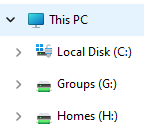
\includegraphics{./images/paste-E035B7C2.png}

H:

\begin{itemize}
\item
  Each person has a part of it
\item
  Documents is a mirror (a link to your H: drive space) \& is backed up
\end{itemize}

G:

\begin{itemize}
\tightlist
\item
  Used to share files with others
\end{itemize}

\hypertarget{culture}{%
\section{Culture}\label{culture}}

We generally like to help each other. That said, the person working for
Claudia before the data analyst position was created received requests
so much so that Claudia had to taper them down.

The data analyst position is more for data projects, but for Megamation
queries. The latter are to be done through Megamation, and tailored
reports there can be made for individuals.

Let Claudia know of any requests that come through, as she will help
prioritize them/decide if they are within the role of the data analyst.

\hypertarget{daily-schedule}{%
\section{Daily Schedule}\label{daily-schedule}}

Work starts at 8:30. Lunch anytime. We generally leave at 4:30.

However this is flexible. If you want to start at 8, and leave at 4,
that's ok. Lunch also does not need to be exactly 1 hour.

\hypertarget{remote-work}{%
\section{Remote Work}\label{remote-work}}

People come in Monday to Friday but the IT departments takes 2
afternoons to work from home in order to focus. They prefer to be away
from the office on these days due to the number of requests they
receive. As a data analyst, you can work from home two full days of the
week in order to be as undistracted as possible.

\hypertarget{sick-leave-vacation-etc.}{%
\section{Sick Leave, Vacation, etc.}\label{sick-leave-vacation-etc.}}

We don't use time-cards anymore. We use
\href{https://m.megamation.com/uog/dlweb.php/O4W_MOBILE_MAIN}{DirectLine
of Megamation}.

Use \textbf{Time Keeping} for inputting vacation, sick leave, etc. NB
Date is set to current day; set it right or it will be
rejected.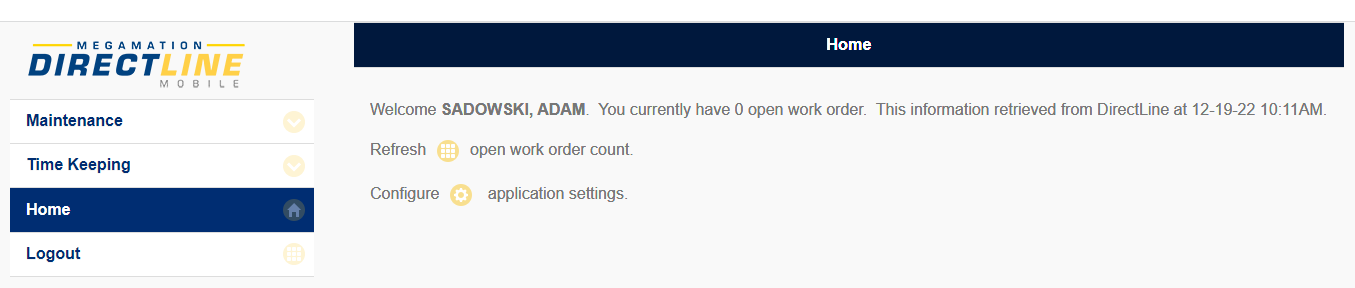
\includegraphics{./images/paste-15194CE2.png}

\hypertarget{notes-on-claudia}{%
\section{Notes on Claudia}\label{notes-on-claudia}}

Claudia often has a closed door as she speaks loud (her words). If she's
on the phone, just poke head in her window \& wave. She will give thumbs
up/down on whether you can come in.

\hypertarget{meetings}{%
\section{Meetings}\label{meetings}}

You can use Outlook to book meeting rooms for individual use using
locations PR meeting room 103 010 106 and 105.

In the stand-alone Outlook application, Scheduling Assistant is great to
see when someone is busy.

For larger meetings, you ca book meeting rooms with Barb.

\hypertarget{computer-administrator-rights}{%
\section{Computer Administrator
Rights}\label{computer-administrator-rights}}

Admin. rights were granted to the desktop in the process of trying to
solve a 0x1 error in Task Scheduler. This error does not stop task
completion, and I solved the error by using UNC paths (as opposed to
drive letters) in the scheduled script. Hence, admin. rights may not
actually be necessary on the desktop.

The following applies if desktop has no administrator rights:

\begin{itemize}
\item
  The desktop will not have administrator rights due to our internal IT
  responsibility
\item
  If needed, you can ask Andrew on Teams and he can remote enter
  passwords
\item
  Admin login is needed for many programs:

  \begin{itemize}
  \item
    Keypirinha is a great program for typing to find files as opposed to
    using File Explorer
  \item
    R command RInno::install\_inno() is needed to turn R Shiny
    applications into standalone executables
  \item
    KeepassXC for password management (or since it was hacked according
    to Chris Payne, though I believe he confused the program with
    another), use PMP (on campus) instead
  \item
    RStudio updates
  \item
    Batch Job Rights in order to fix Windows Taskscheduler error 0x1

    \begin{itemize}
    \item
      For rights, alert IT to
      \url{https://www.urtech.ca/2019/06/solved-this-task-requires-that-the-user-account-specified-has-log-on-as-batch-job-rights/}
    \item
      For fixing the 0x1 error, see
      \url{https://redstapler.co/fix-task-scheduler-0x1-error/}
    \end{itemize}
  \end{itemize}
\end{itemize}

\hypertarget{equipment}{%
\section{Equipment}\label{equipment}}

\hypertarget{clothing}{%
\subsection{Clothing}\label{clothing}}

The stockroom can supply toques, shirts (polos, dress), sweaters,
fleece, and jackets. The stockroom supplies the university with a lot.
COVID-19 PPE was supplied through the stockroom, and departments
realized what else the stockroom can provide. Hence business boomed.

Claudia can approve items you would like.

\hypertarget{laptop}{%
\subsection{Laptop}\label{laptop}}

IT will provide you with a laptop.

\hypertarget{chair}{%
\subsection{Chair}\label{chair}}

If a new chair is needed and apporved by Chris or Claudia, you may book
an appointment with Occupational Health \& Wellness for a chair fitting.

Adam was fitted with a Steelcase Leap Feb.~2, 2023.

\hypertarget{humidifier}{%
\subsection{Humidifier}\label{humidifier}}

Personal humidifiers can also be supplied if the building's relative
humidity cannot be increased in the winter to 40-50\%.

\bookmarksetup{startatroot}

\hypertarget{sec-megamation}{%
\chapter{Megamation}\label{sec-megamation}}

\hypertarget{access-instructions}{%
\section{Access Instructions}\label{access-instructions}}

\begin{enumerate}
\def\labelenumi{\arabic{enumi}.}
\item
  IT will create your Megamation account.
\item
  \textbf{Citrix Workspace App} needs to be downloaded. It is a secure
  interface to the webpage where Megamation lives. Download it from
  \href{https://www.citrix.com/downloads/workspace-app/}{here}.
\item
  Click ``Citrix Workspace app {[}XXXX{]} for Windows''. Install it and
  do \textbf{not} click any optional boxes like ``Add account''.
  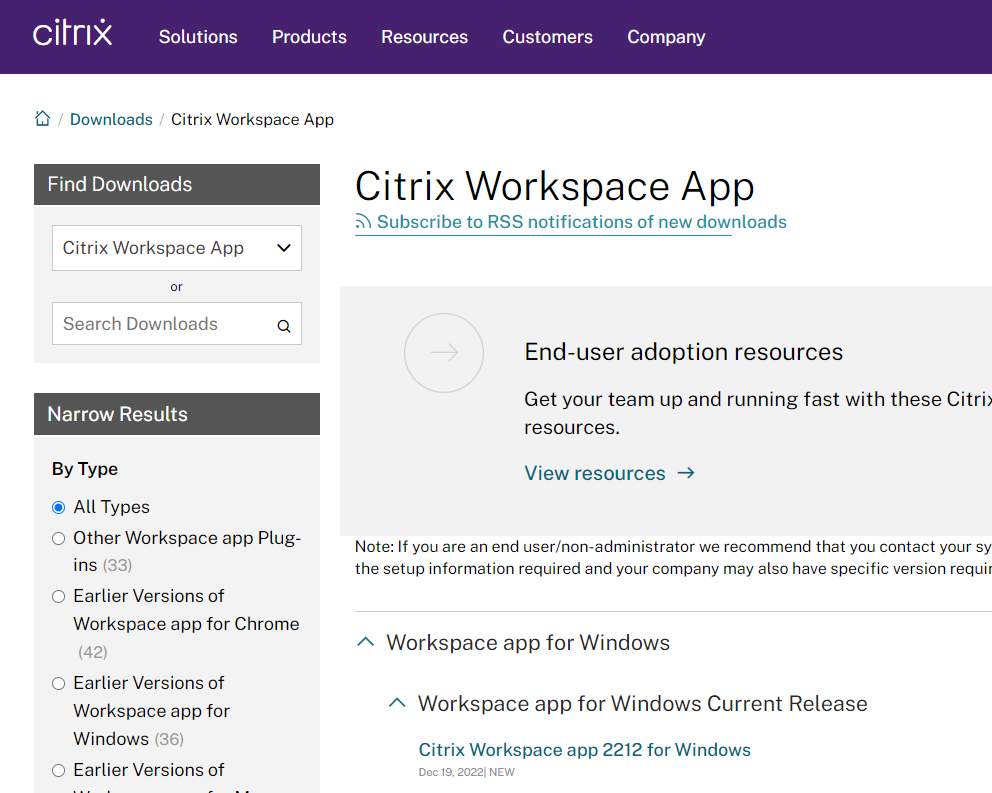
\includegraphics{./images/paste-9F18CD79.png}
\item
  Add https://sso.megamation.com/ to your ``Chrome Settings - Cookies -
  Always clear cookies when windows are closed''. See the very bottom of
  this screenshot: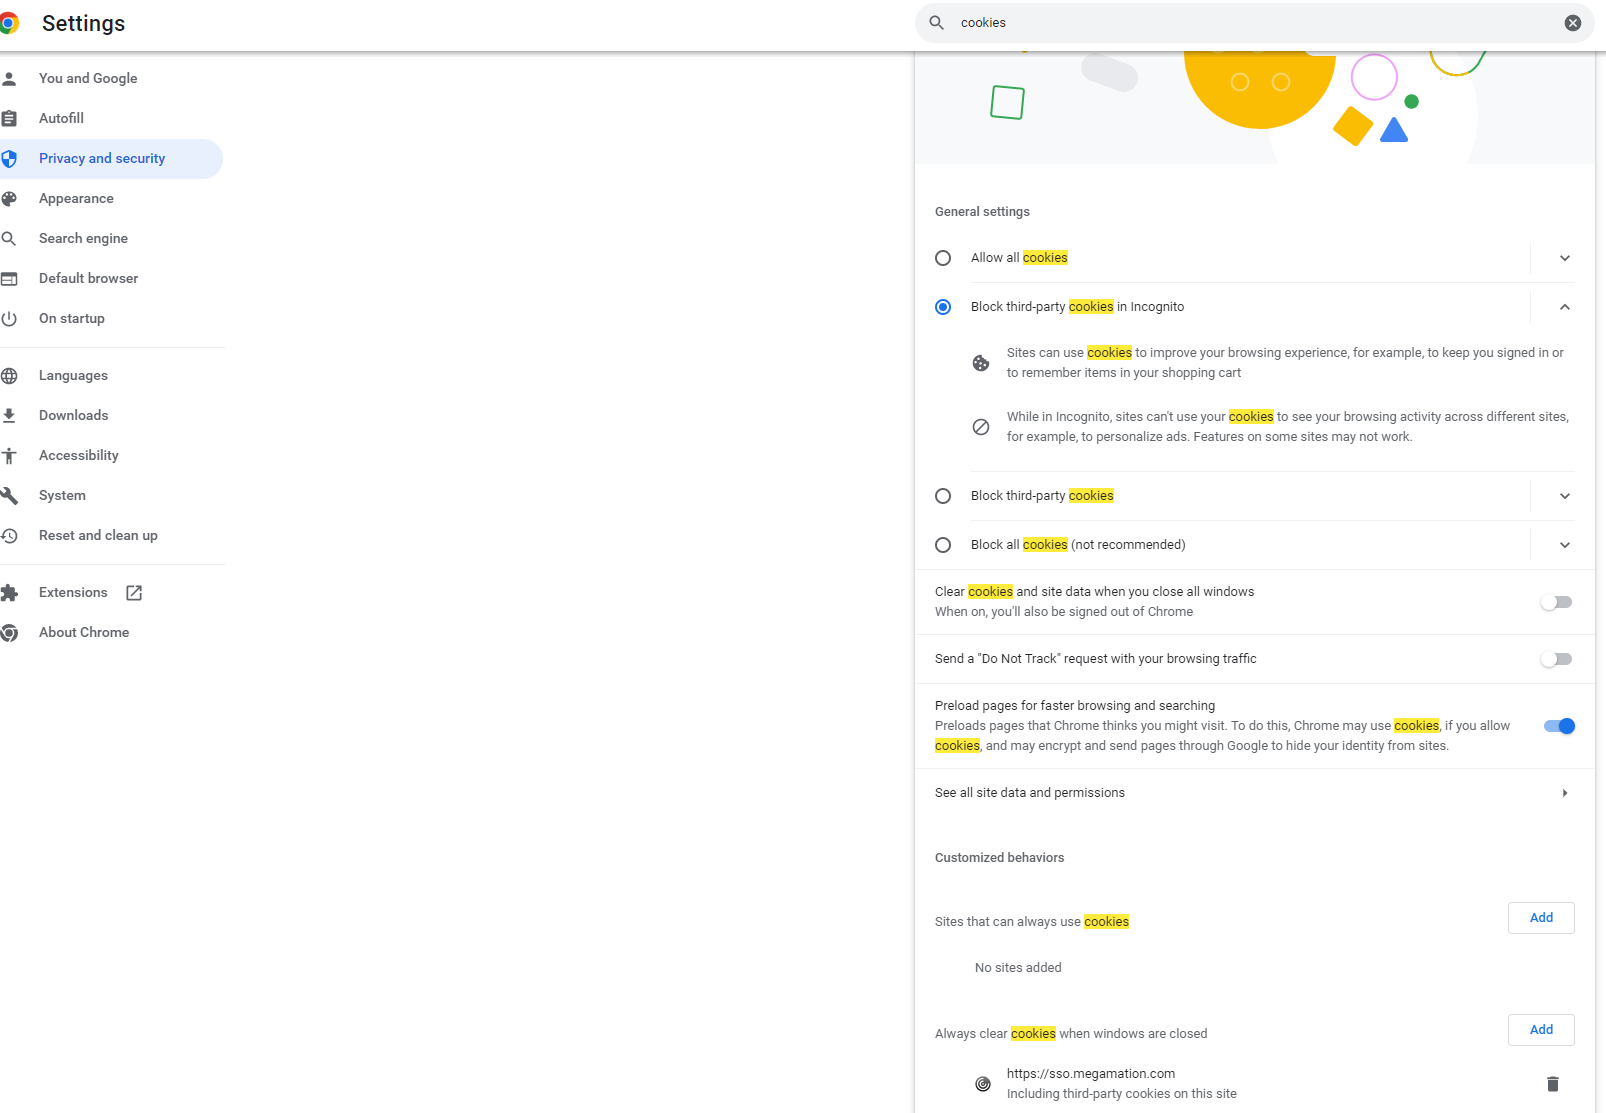
\includegraphics{./images/paste-B97C5881.png}
\end{enumerate}

{\marginnote{\begin{footnotesize}The need for clearing cookies is we
need a new session id each time we start Chrome.\end{footnotesize}}}

\begin{enumerate}
\def\labelenumi{\arabic{enumi}.}
\setcounter{enumi}{4}
\tightlist
\item
  Using the link in 4., access Citrix via a private browser
  (e.g.~Chrome's Incognito Mode) to avoid a cache. You will see this
  \href{https://sso.megamation.com/uog}{web page}.
\end{enumerate}

{\marginnote{\begin{footnotesize}The need for the incognito window has
to do with CCS encryption where if we get kicked out of UofG's Central
login we cannot log back into Megamation.\end{footnotesize}}}

\begin{enumerate}
\def\labelenumi{\arabic{enumi}.}
\setcounter{enumi}{5}
\item
  Click \emph{D} in this part of the webpage:

  
\includegraphics{./images/paste-EF9D2C62.png}
\item
  This application will open on your taskbar with the icon
  
\includegraphics{./images/paste-F823AE87.png}
\item
  NB \textbf{Never} click the outermost X (very top right) on the
  following screenshot of a Citrix instance; it severs connection to the
  database and IT will need to reinstate the connection.

  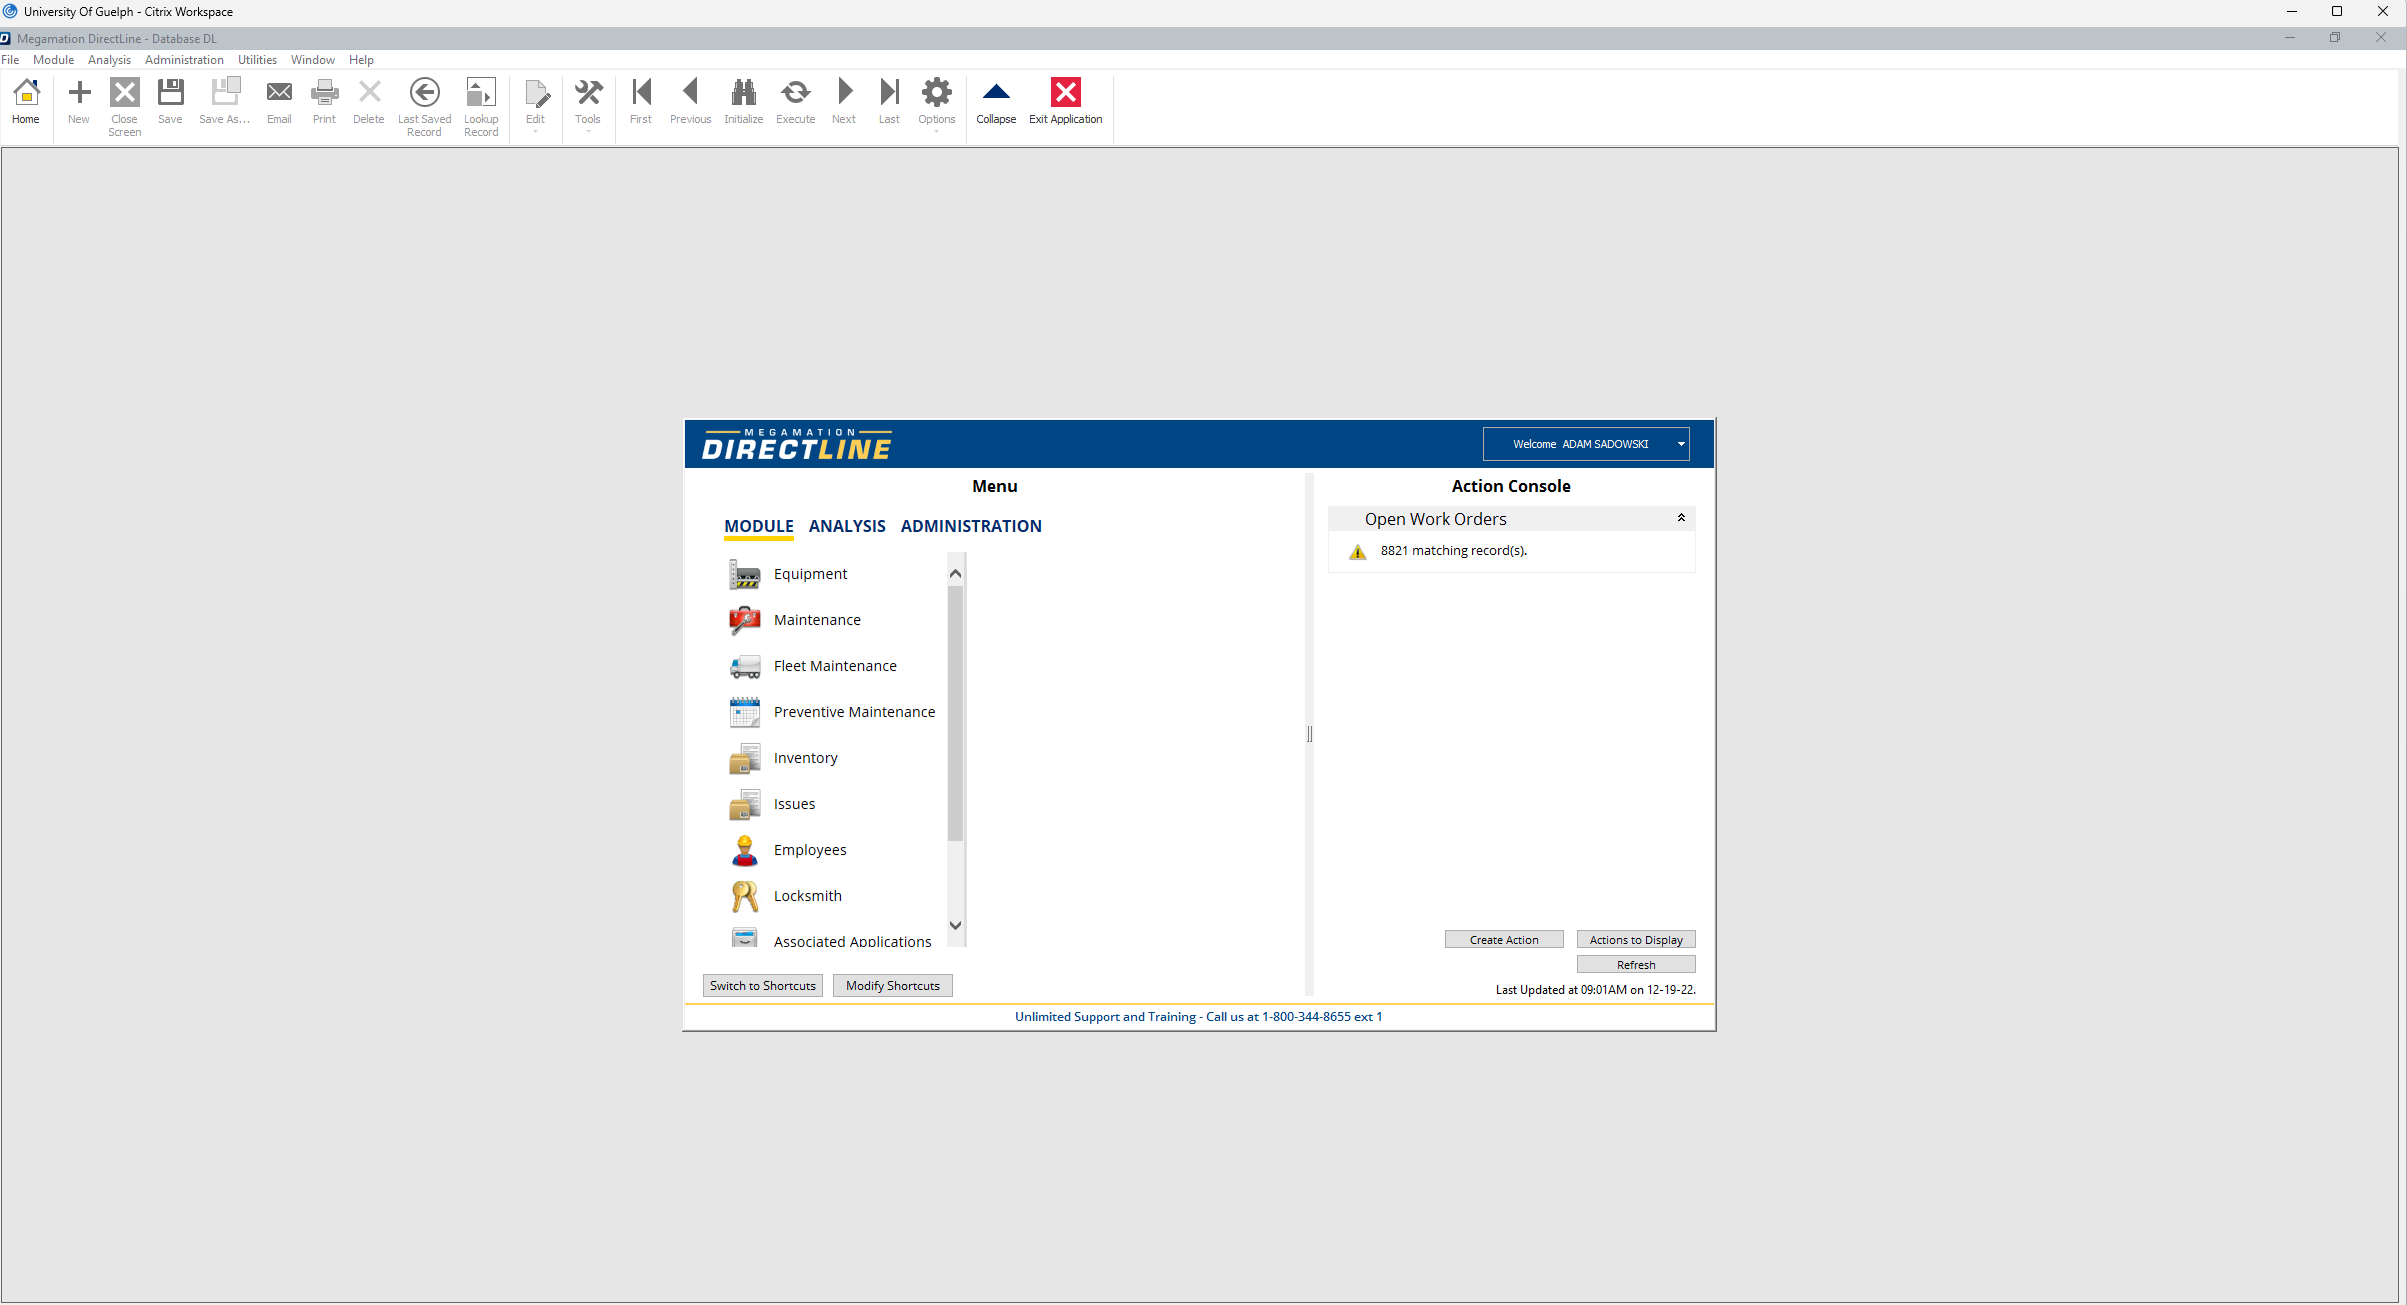
\includegraphics{./images/paste-5F3C0CAF.png}
\end{enumerate}

\hypertarget{megamation-export-example}{%
\section{Megamation Export Example}\label{megamation-export-example}}

\hypertarget{define-the-export}{%
\subsection{Define the export}\label{define-the-export}}

Click ``Analysis'' and then ``Export Definition Wizard''.

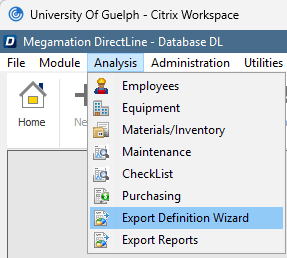
\includegraphics{./images/paste-6E3647FD.png}

Click ``\uline{N}ext''.

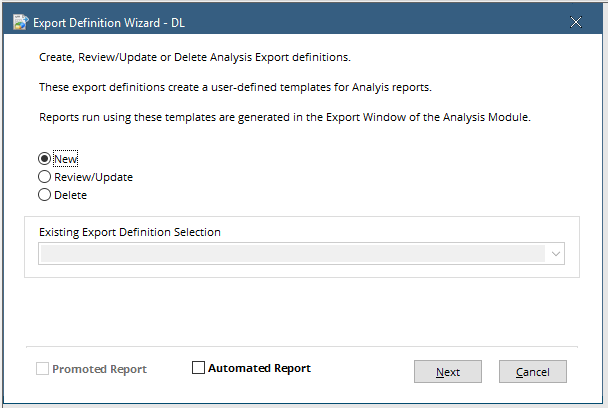
\includegraphics{./images/paste-20DE5D3A.png}

Select a table.

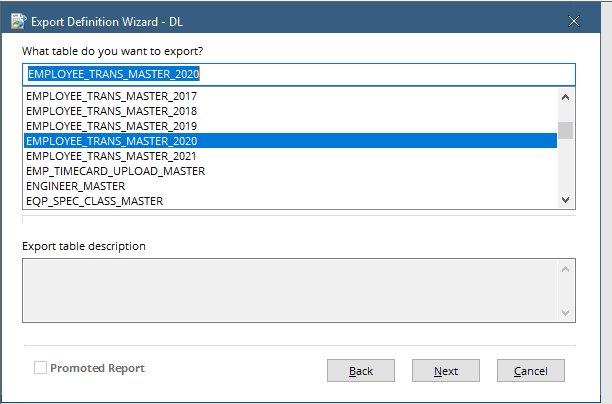
\includegraphics{./images/paste-63EB2380.png}

Click ``\uline{N}ext'', and then ``Add''. Add among the fields from the
table that pops up on the right.

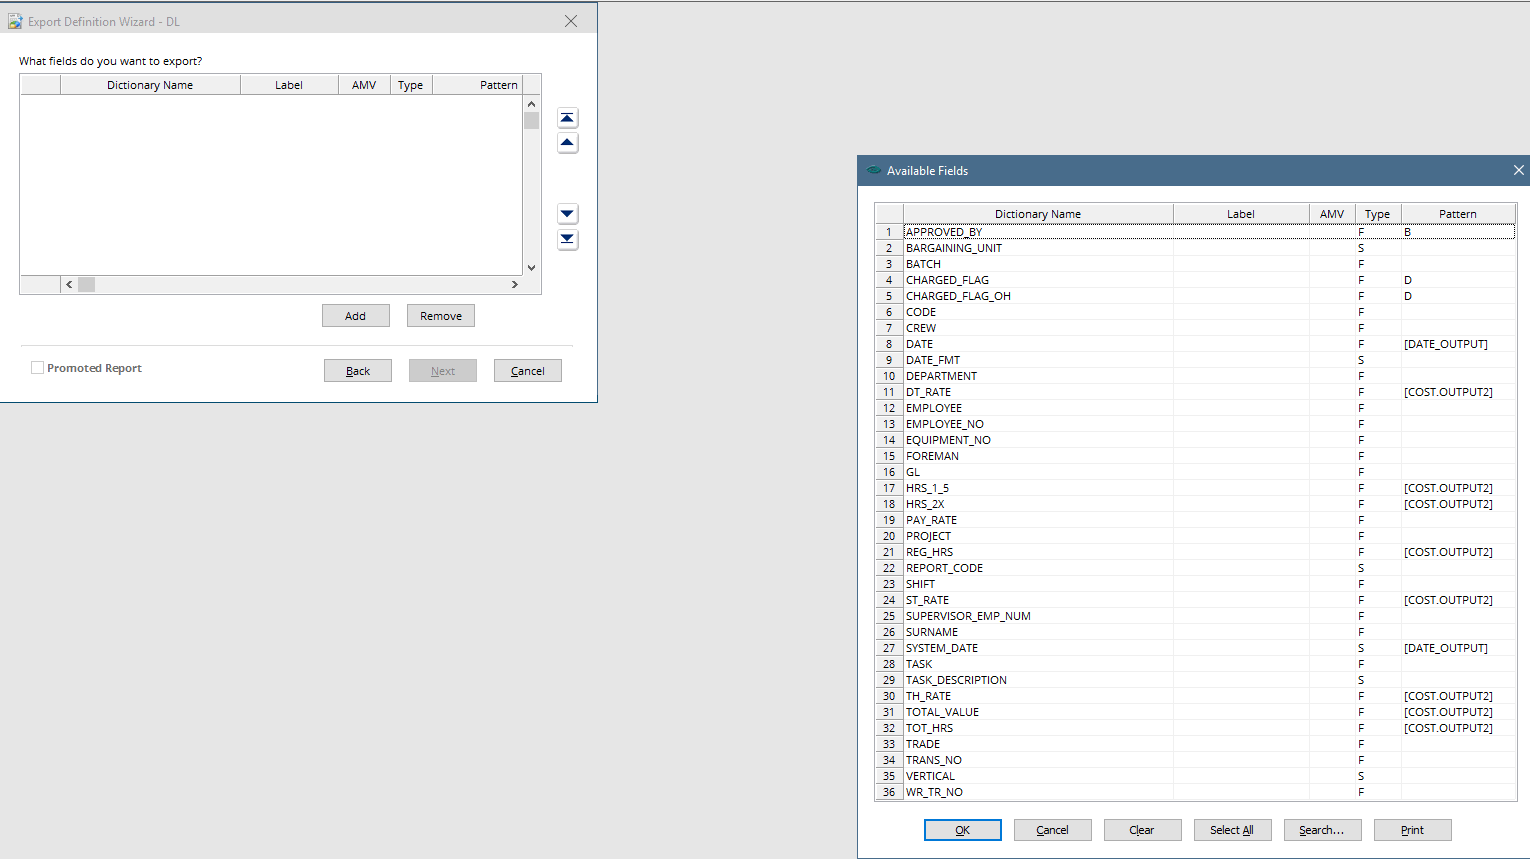
\includegraphics{./images/paste-87EAAAE5.png}

Click ``\uline{N}ext'' again and again\ldots{} You can select some
options if you want.

\hypertarget{do-the-export}{%
\subsection{Do the export}\label{do-the-export}}

Click ``Analysis'' and then ``Export Reports''.

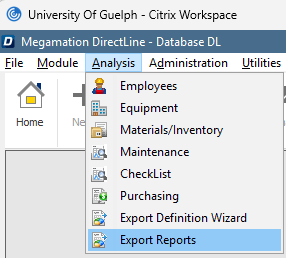
\includegraphics{./images/paste-4B84E0CD.png}

Click ``Export'' at bottom right. Click off ``Auto-format Spreadsheet''
if you want a faster export.

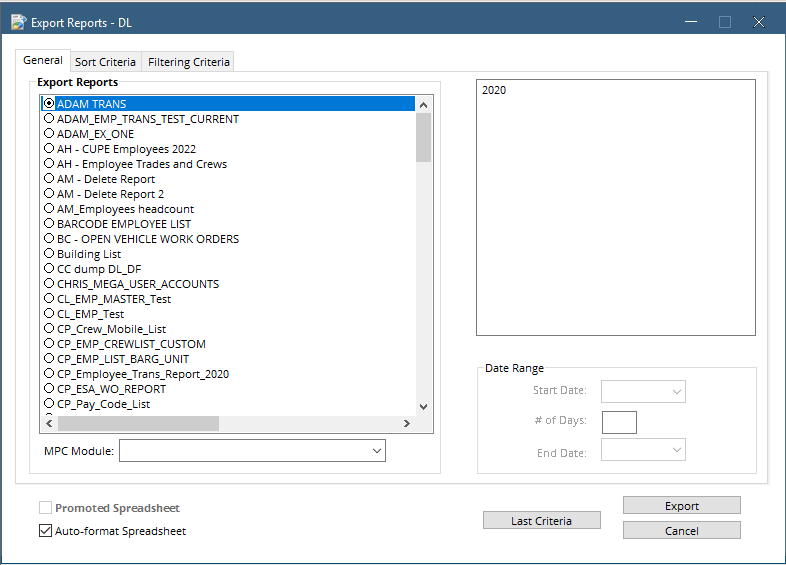
\includegraphics{./images/paste-CA669F29.png}
{\marginnote{\begin{footnotesize}NB for big files: the Excel file that
pops up after clicking Export'' may not be ready and may still be
populating. This is why we use ``Automated Report'' (second image under
\textbf{Define the export}) for big exports. ``Automated Report'' will
do automatically do the export in the morning and save it. If not using
``Automated Report'', make sure to save the Excel pop-up file before
closing.\end{footnotesize}}}

Click ``Utilities'' and the following.

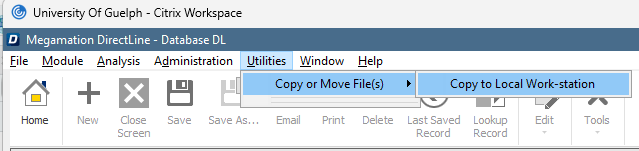
\includegraphics{./images/paste-CA9DAE7B.png}

Files can then be selected to be emailed or downloaded.

\hypertarget{checking-work-orders}{%
\section{Checking Work Orders}\label{checking-work-orders}}

If Steve asks about a work order, Evan usually follows these steps:

\begin{enumerate}
\def\labelenumi{\arabic{enumi}.}
\item
  Export Request

  \begin{itemize}
  \item
    Pick ML WO Inquiry (Matt Laury Work Order)
  \item
    Filter by

    \begin{itemize}
    \item
      Building number: e.g.~72
    \item
      Status: CL is closed, so filter out CL if you are looking for open
      orders
    \end{itemize}
  \item
    Export
  \item
    Sort and look for, say, mold in the Work Description
  \item
    Find work order number e.g.~192331
  \end{itemize}
\item
  Work Order Completion

  \begin{itemize}
  \item
    Enter the work order number
  \item
    See if it was scheduled and when it was issued

    \begin{itemize}
    \tightlist
    \item
      There is no way AFAWK to get date it was scheduled vs.~issued
    \end{itemize}
  \end{itemize}
\end{enumerate}

\hypertarget{notes-on-filters}{%
\section{Notes on Filters}\label{notes-on-filters}}

\begin{itemize}
\item
  Fund

  \begin{itemize}
  \item
    100 series: Core of the university
  \item
    300 series: ???
  \item
    500 series: Ancillary

    \begin{itemize}
    \item
      Residences
    \item
      Hospitality
    \item
      Particular research spaces
    \end{itemize}
  \end{itemize}
\item
  Unit

  \begin{itemize}
  \tightlist
  \item
    I.e. department. ``XX'' suffix is the set of all suffixes. ``99'' is
    general but does not contain other sets.
  \end{itemize}
\item
  Grant

  \begin{itemize}
  \tightlist
  \item
    E.g. if a researcher needs something to be fixed using their grant
    money.
  \end{itemize}
\item
  Project

  \begin{itemize}
  \item
    Unique code.
  \item
    Projects starting with 8 are internal and will not have a grant
    number.
  \end{itemize}
\end{itemize}

\part{Tasks}

\hypertarget{esa-online-submissions}{%
\chapter{ESA Online Submissions}\label{esa-online-submissions}}

Goal: Successfully upload our work orders to ESA Online.

Currently a Megamation report is generated as below. Remember to specfiy
the start and end date at the bottom right.

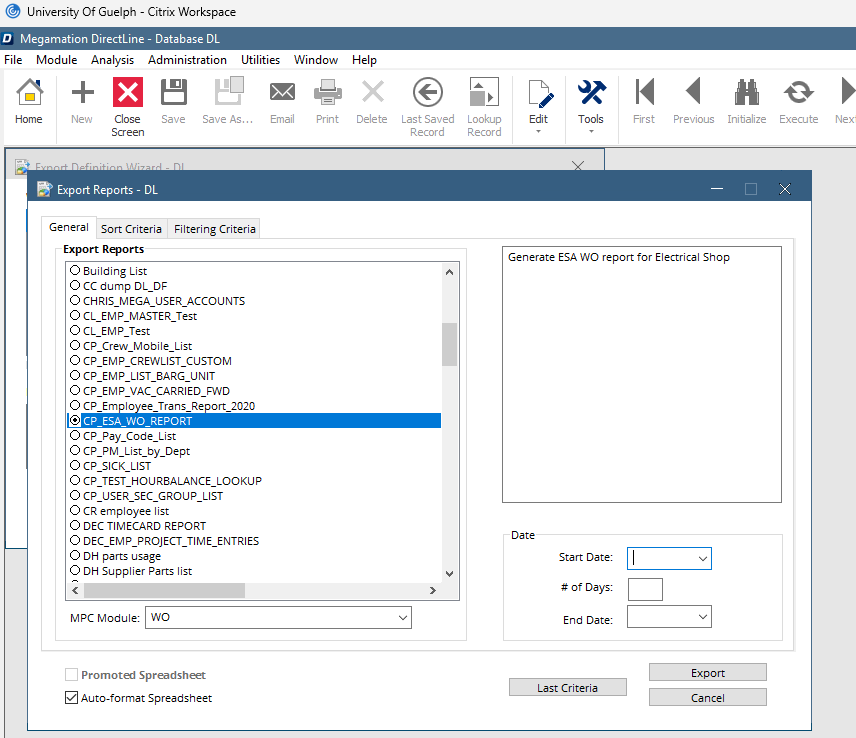
\includegraphics{./images/paste-FF17F682.png}

This file is to be placed in a shared folder.

An R script will attach and prepare the data in the format necessary for
upload to ESA Online.

This link will take you to the ESA website:
\url{https://cssl.esasafe.com/CSS} Do not google for it, as you may end
up at a very similar looking portal, where the only difference is the
phrase underneath the title ``esa online''. The right looking portal
says ``CSS Portal'' there, as shown below.

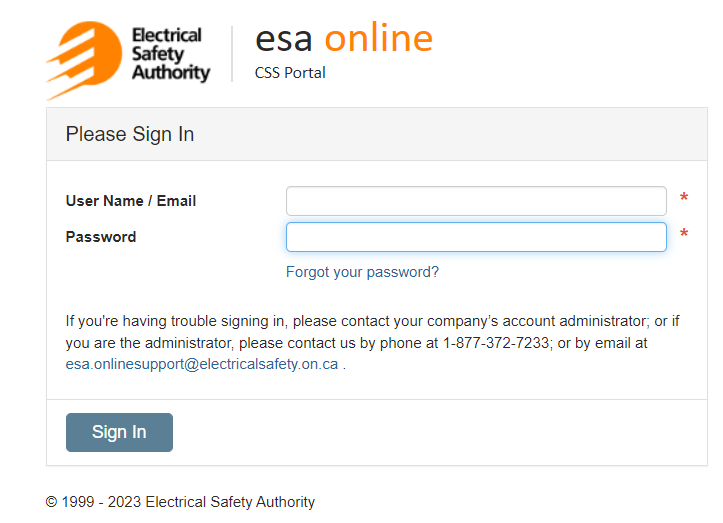
\includegraphics{./images/paste-AD90C473.png}

Logging in will bring you to

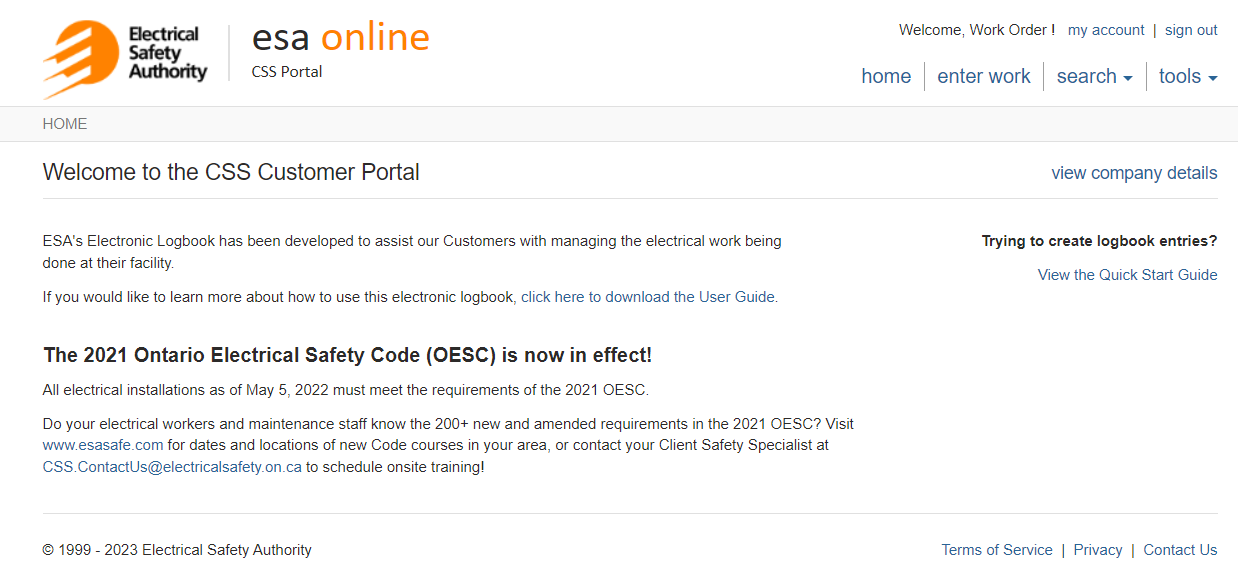
\includegraphics{./images/paste-899B5AC7.png}

Hit ``tools'' on the top right, then ``Logbook Entry Uploads''. At the
next screen below, click ``Browse\ldots{}'', find and select the
aforementioned file. Hit ``Upload''. That's it!

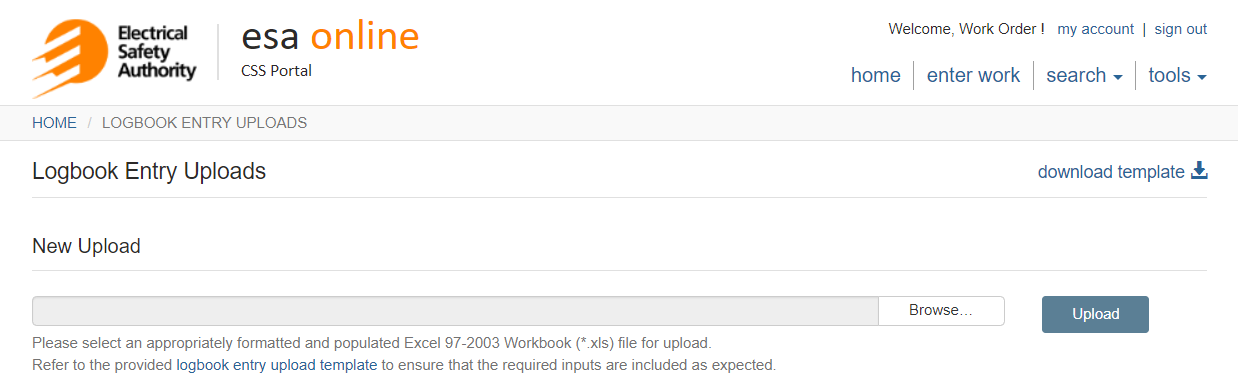
\includegraphics{./images/paste-7F4BC4D4.png}

\part{Quality Control}

\hypertarget{data-quality}{%
\chapter{Data Quality}\label{data-quality}}

\hypertarget{review}{%
\section{Review}\label{review}}

\begin{itemize}
\item
  Using package \texttt{assertr} (from
  \url{https://cran.r-project.org/web/packages/assertr/vignettes/assertr.html})

  \begin{itemize}
  \item
    \texttt{verify} for

    \begin{itemize}
    \tightlist
    \item
      data frames e.g.~does a data frame have names code and department?
      \texttt{verify(has\_all\_names("code",\ "department"))}
    \end{itemize}
  \item
    \texttt{assert}

    \begin{itemize}
    \item
      for variables and without interaction e.g.

      \begin{itemize}
      \item
        \texttt{assert(within\_bounds(0,\ Inf),\ some\_column)}
      \item
        \texttt{assert(in\_set(known\_levels),\ some\_column)}
      \item
        \texttt{is\_not\_empty\ \textless{}-\ function(x)\ if(x\ !=\ "")\ return(TRUE)}

        \begin{itemize}
        \tightlist
        \item
          \texttt{assert(is\_not\_empty,\ some\_column)}
        \end{itemize}
      \end{itemize}
    \end{itemize}
  \item
    \texttt{insist}

    \begin{itemize}
    \item
      for variables after interacting with them e.g.

      \begin{itemize}
      \item
        \texttt{insist(within\_n\_mads(3),\ some\_column)}

        \begin{itemize}
        \item
          NB ``The problem with \texttt{within\_n\_sds} is the mean and
          standard deviation are so heavily influenced by outliers,
          their very presence will compromise attempts to identify them
          using these statistics. In contrast with
          \texttt{within\_n\_sds}, \texttt{within\_n\_mads} uses the
          robust statistics, median, and median absolute deviation, to
          identify potentially erroneous data points.''
        \item
          How to build custom predicate generators:

\begin{Shaded}
\begin{Highlighting}[]
\NormalTok{within\_n\_iqrs }\OtherTok{\textless{}{-}} \ControlFlowTok{function}\NormalTok{(n, ...)\{}
  \ControlFlowTok{function}\NormalTok{(a\_vector)\{}
\NormalTok{    the\_median }\OtherTok{\textless{}{-}} \FunctionTok{median}\NormalTok{(a\_vector)}
\NormalTok{    the\_iqr }\OtherTok{\textless{}{-}} \FunctionTok{IQR}\NormalTok{(a\_vector)}
    \FunctionTok{within\_bounds}\NormalTok{((the\_median}\SpecialCharTok{{-}}\NormalTok{the\_iqr}\SpecialCharTok{*}\NormalTok{n), (the\_median}\SpecialCharTok{+}\NormalTok{the\_iqr}\SpecialCharTok{*}\NormalTok{n), ...)}
\NormalTok{  \}}
\NormalTok{\}}

\NormalTok{mtcars }\SpecialCharTok{|\textgreater{}} 
  \FunctionTok{insist}\NormalTok{(}\FunctionTok{within\_n\_iqrs}\NormalTok{(}\DecValTok{5}\NormalTok{), mpg)  }\SpecialCharTok{|\textgreater{}} 
  \FunctionTok{group\_by}\NormalTok{(cyl) }\SpecialCharTok{|\textgreater{}} 
  \FunctionTok{summarise}\NormalTok{(}\AttributeTok{avg.mpg =} \FunctionTok{mean}\NormalTok{(mpg))}
\end{Highlighting}
\end{Shaded}
        \end{itemize}
      \end{itemize}
    \end{itemize}
  \item
    \texttt{insist\_rows}

    \begin{itemize}
    \item
      for rows with interaction e.g.

      \begin{itemize}
      \item
        \texttt{insist\_rows(maha\_dist,\ within\_n\_mads(3),\ dplyr::everything())}

        \begin{itemize}
        \tightlist
        \item
          NB ``\texttt{maha\_dist} computes the average mahalanobis
          distance (kind of like multivariate z-scoring for outlier
          detection) of each row from the whole data set. The big idea
          is that in the resultant vector, big/distant values are
          potential anomalous entries.''
        \end{itemize}
      \end{itemize}
    \end{itemize}
  \item
    \texttt{chain\_start} and \texttt{chain\_end} for chains of
    assertions

    \begin{itemize}
    \item
      e.g.

\begin{Shaded}
\begin{Highlighting}[]
\FunctionTok{library}\NormalTok{(assertr)}

\NormalTok{our.data }\OtherTok{\textless{}{-}}\NormalTok{ mtcars}
\NormalTok{our.data}\SpecialCharTok{$}\NormalTok{mpg[}\DecValTok{5}\NormalTok{] }\OtherTok{\textless{}{-}}\NormalTok{ our.data}\SpecialCharTok{$}\NormalTok{mpg[}\DecValTok{5}\NormalTok{] }\SpecialCharTok{*} \SpecialCharTok{{-}}\DecValTok{1}

\NormalTok{our.data  }\SpecialCharTok{|\textgreater{}} 
  \FunctionTok{chain\_start}\NormalTok{()  }\SpecialCharTok{|\textgreater{}} 
  \FunctionTok{assert}\NormalTok{(}\FunctionTok{within\_bounds}\NormalTok{(}\DecValTok{0}\NormalTok{, }\ConstantTok{Inf}\NormalTok{), mpg) }\SpecialCharTok{|\textgreater{}} 
  \FunctionTok{insist}\NormalTok{(}\FunctionTok{within\_n\_sds}\NormalTok{(}\DecValTok{4}\NormalTok{), mpg) }\SpecialCharTok{|\textgreater{}} 
  \FunctionTok{chain\_end}\NormalTok{()}
\end{Highlighting}
\end{Shaded}

\begin{verbatim}
There are 2 errors across 2 verbs:
- 
    verb redux_fn             predicate column index value
1 assert       NA within_bounds(0, Inf)    mpg     5 -18.7
2 insist       NA       within_n_sds(4)    mpg     5 -18.7
\end{verbatim}

\begin{verbatim}
Error: assertr stopped execution
\end{verbatim}
    \end{itemize}
  \end{itemize}
\end{itemize}

\hypertarget{data-dictionary-building}{%
\section{Data Dictionary Building}\label{data-dictionary-building}}

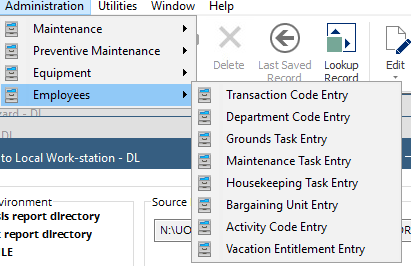
\includegraphics{./images/paste-7368A84B.png}

Note for Export Report:

\begin{itemize}
\item
  S Type vs F: controlled vs calculated
\item
  pattern is basically like class
\end{itemize}

\hypertarget{code-quality}{%
\chapter{Code Quality}\label{code-quality}}

\begin{itemize}
\item
  Controls

  \begin{itemize}
  \item
    R packages for documentation of data and code

    \begin{itemize}
    \item
      Standardize function
      names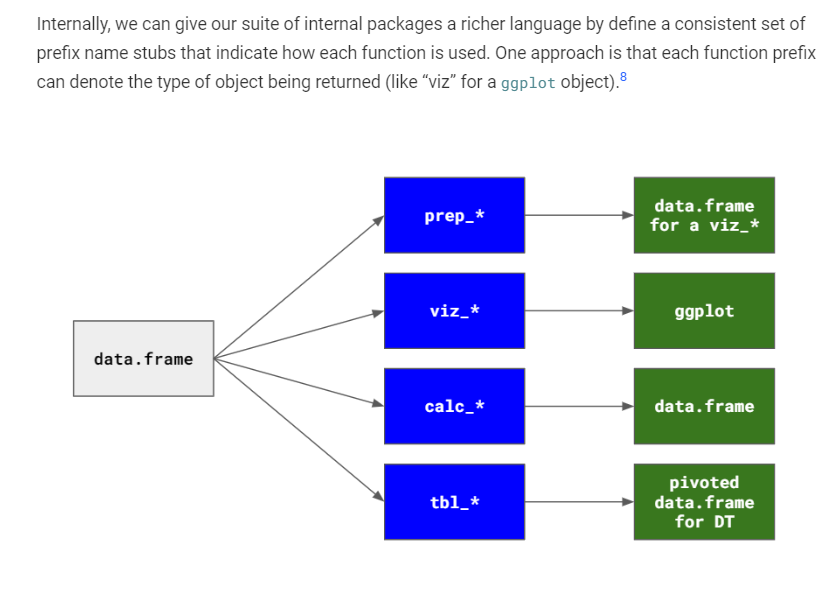
\includegraphics{./images/paste-F452E92E.png}
    \item
      Read Wickham's Packages: use\_package\_doc() and edit it to add
      imports, whether all functions by (\textbf{import?}) or specific
      by use\_import\_from()
    \end{itemize}
  \item
    renv for app environment/dependency control
  \item
    git for version control
  \item
    tests for automated code control

    \begin{itemize}
    \item
      unit (for individual functions)
    \item
      integration (for interactions between reactives)
    \item
      functional (for end-to-end experience from a browser)
    \item
      load (for withstanding traffic)
    \end{itemize}
  \item
    continuous integration for change control (requires code control and
    version control) - notifies if changes break or will break an app
  \end{itemize}
\item
  Organization

  \begin{itemize}
  \item
    Put large functions (and any smaller helper functions that they
    need) into their own \texttt{R/\{function-name\}.R} file
  \item
    For complicated apps, read the
    \href{https://engineering-shiny.org/}{``Engineering Shiny''} book
    and use the accompanying
    \href{https://thinkr-open.github.io/golem/}{golem} package
  \item
    If developing a lot of Shiny apps within your organisation, improve
    cross-app consistency by putting functions in a shared package
  \item
    With a long reactive (say \textgreater10 lines), consider pulling it
    out into a separate function that does not use any reactivity. This
    has two advantages:

    \begin{itemize}
    \item
      It is much easier to debug and test code if it can be partitioned
      so that reactivity lives inside of \texttt{server()}, and complex
      computation lives in functions.
    \item
      When looking at a reactive expression or output, there's no way to
      easily tell exactly what values it depends on, except by carefully
      reading the code block. A function definition, however, shows
      exactly what the inputs are.
    \item
      The key benefits of a function in the UI tend to be around
      reducing duplication. The key benefits of functions in a server
      tend to be around isolation and testing.
    \end{itemize}
  \end{itemize}
\end{itemize}

\bookmarksetup{startatroot}

\hypertarget{servers}{%
\chapter{Servers}\label{servers}}

\hypertarget{platform-for-interactive-applications}{%
\subsection{Platform for Interactive
Applications}\label{platform-for-interactive-applications}}

There are
\href{https://posit.co/products/open-source/shinyserver/?_ga=2.218758425.1435543973.1677605377-1975567833.1670879814}{three
options for hosting applications (scroll to bottom for comparison).} The
center option is 50\% off for academic institutions.


\includegraphics{./images/paste-B7CB568F.png}

\hypertarget{no-cash-cost-and-internal}{%
\subsubsection{No Cash Cost and
Internal}\label{no-cash-cost-and-internal}}

The left-most option is the one we host ourselves. There are two options
to do this.

\begin{enumerate}
\def\labelenumi{\arabic{enumi}.}
\tightlist
\item
  On a Linux distribution using the
  \href{https://docs.posit.co/shiny-server/}{administrator's guide.} If
  we want applications to be used by multiple people at the same time
  (e.g.~Claudia and Kristen), this is not the best.
  \href{https://stackoverflow.com/questions/59169546/how-do-we-configure-shinyserver-open-source-to-support-concurrent-users}{A
  response on StackOverflow regarding concurrent use} describes how
  ``with this option you can find your users hitting multiple times the
  inputs or interactive outputs and the app seeming stuck''. But this
  should be fine for now. We can co-ordinate to have one person at a
  time using each application.
\item
  \href{https://www.shinyproxy.io/}{Using Java and Docker containers}.
  We get LDAP authentication, no limits on concurrent usage. I'm not
  experienced with Docker but happy to learn.
\end{enumerate}

This may be cash-less and avoid requiring approval from CCS, but it
creates hours (and thus costs) of set-up, maintenance, de-bugging, etc.

\hypertarget{cheap-and-external}{%
\subsubsection{Cheap and External}\label{cheap-and-external}}

I am already using the right-most option \textbf{Shinyapps.io}. This is
hosting the
\href{https://physical-resources.shinyapps.io/shovelapp/}{snow shovel
routes dashboard that self-updates daily.} The free option has no
user-authentication. I.e. this link is available to anyone. If we pay
\textbf{\$100/month}, we can have user-authentication. The data is still
hosted on an external server by the company Posit. (This company
produces the open-source tools for R. Services like these is how they
make money.) There is no letter of standing of security procedures apart
from
\href{https:/docs.posit.co/shinyapps.io/security-and-compliance.html}{a
page on security compliance.}

\hypertarget{not-cheap-and-external-but-comprehensive}{%
\subsubsection{Not Cheap and External, But
Comprehensive}\label{not-cheap-and-external-but-comprehensive}}

The center option \textbf{\$7500/year (academic pricing)} is a
comprehensive service, where not just hosting applications is possible,
but also:

\begin{itemize}
\item
  Scheduling and managing repeated tasks/jobs more easily than using
  Windows Task Scheduler or Cron.
\item
  Providing a website for us where all static reports, books, and
  parameterized reports I generate are organized, shared, time-stamped,
  versioned, etc. For parameterized reports, users apart from me can
  adjust parameters, like below. This is more efficient than someone
  asking for me to re-run and share a report with different parameters.

  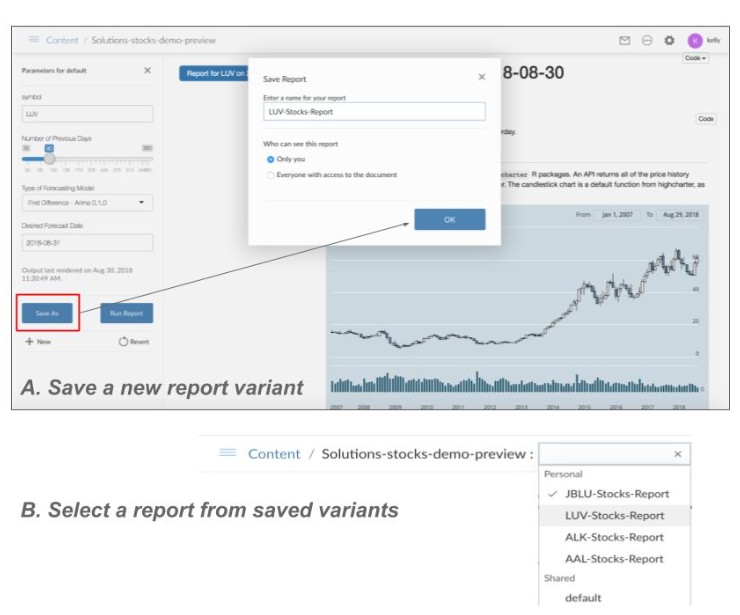
\includegraphics{./images/paste-5C8D338D.png}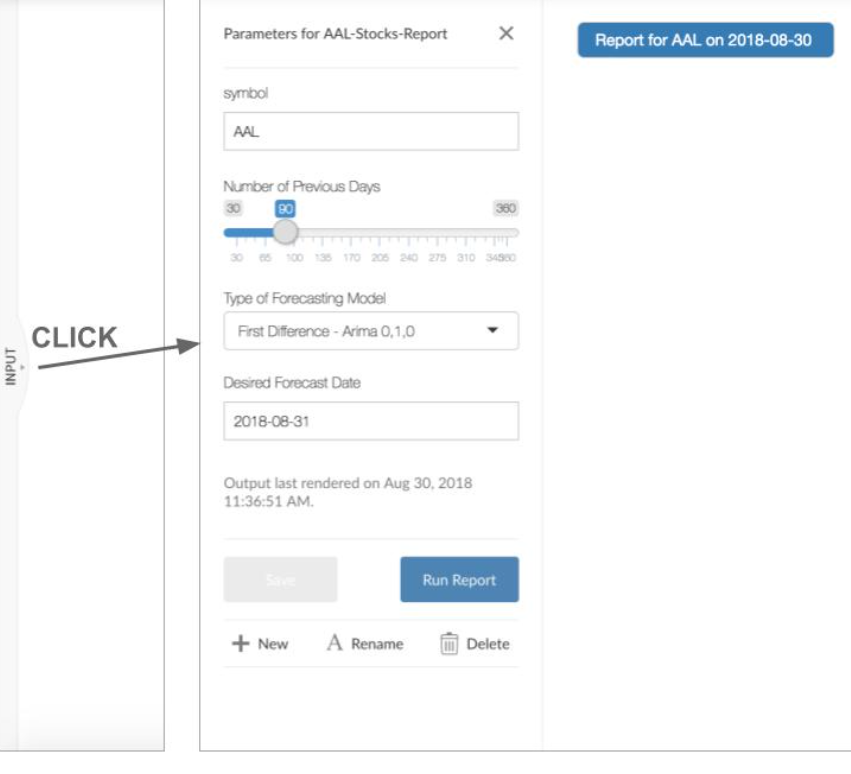
\includegraphics{./images/paste-6201854A.png}
\item
  User access limits, automatic emailing.
\item
  Again, the company Posit hosts the data and this is the
  \href{https:/docs.posit.co/shinyapps.io/security-and-compliance.html}{page
  on security compliance.}
\end{itemize}

\emph{A last option is to make the applications into executable programs
through \href{https://github.com/chasemc/electricShine}{Electron} and
RInno but these projects are dormant/or have mixed reviews regarding
success.}

\hypertarget{a-way-to-access-a-server-with-up-to-date-data}{%
\subsection{A Way to Access (a Server with) Up-To-Date
Data}\label{a-way-to-access-a-server-with-up-to-date-data}}

Currently when I need up-to-date data, I ask Li to set-up automatic
emails. This works for small exports like the CP\_ESA report:

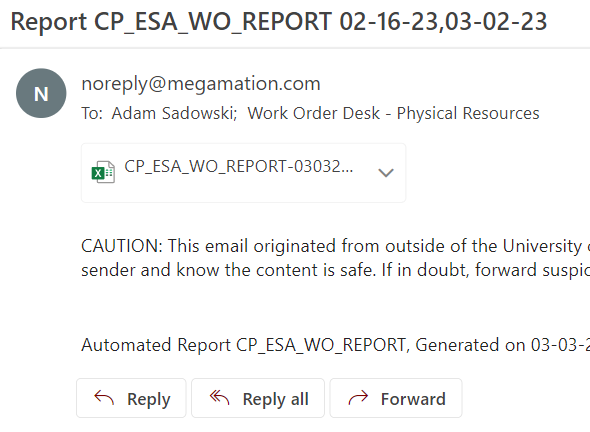
\includegraphics{./images/paste-AF654981.png}

I download it, throw it into a folder, and run code to process it.

I'm concerned this method will not scale over-time. For two reasons:

\begin{enumerate}
\def\labelenumi{\arabic{enumi}.}
\tightlist
\item
  If an application or report relies on up-to-date data like the
  \href{https://physical-resources.shinyapps.io/shovelapp/}{snow shovel
  routes dashboard that self-updates daily}, it is more set-and-forget,
  self-sustaining, and less error-prone to have data hosted somewhere.
  In the case of the shovel routes, data is hosted on Qualtrics'
  servers.
\item
  Certain files I need may be too large or add complexity to code in
  order to avoid duplication. E.g. 2023's employee sick transactions,
  bi-weekly for an application so Stephany can see everyone's sick
  occasions. Unlike the ESA data, I cannot receive only 2-weeks worth of
  data and throw it into a folder. Transaction data gets regularly
  corrected retroactively. I need the full 2023 data, regularly.
\end{enumerate}

Basically a similar code interface to Qualtrics' but for Directline
would be best. E.g. when I interface to Qualtrics, I can query data
using an R function like

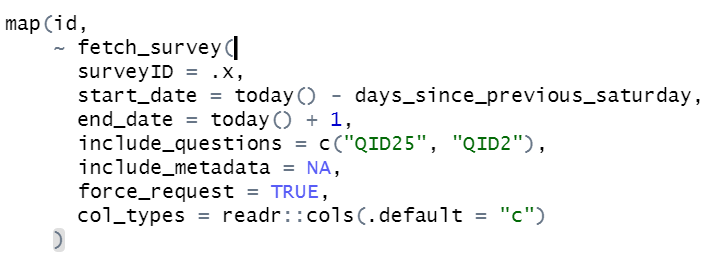
\includegraphics{./images/paste-DA634CE0.png}

If it weren't for this function, I'd need to manually use the Qualtrics'
website to download data, filter it there or elsewhere, pick the columns
there or elsewhere, each day.

\hypertarget{megamation-api}{%
\subsubsection{Megamation API}\label{megamation-api}}

They said we can write programs to pull data from their API into our own
SQL database on-premise. I am not familiar with SQL, besides that all
the filtering, data-cleaning done with SQL code is covered by R. We may
not even need MySQL. Perhaps just R code to be able to pull data
straight from Directline.

They mentioned these limits:

\begin{itemize}
\item
  Max. load of API is 50MB
\item
  Request can't exceed 120 seconds
\end{itemize}

They don't concern me, as for now I don't see us pulling big data
through the API.

\bookmarksetup{startatroot}

\hypertarget{to-do}{%
\chapter{To-Do}\label{to-do}}

\begin{itemize}
\tightlist
\item
  Ask for a Data folder in Groups, with permissions only for oneself,
  and subfolders can have more permissions
\end{itemize}

transApp:

\begin{itemize}
\tightlist
\item
  Add error messages, and req()
\item
  Add a ``render'' button to transApp to avoid unnecessary computations
  due to ``full reactivity''
\item
  Use an employee master as the data for UI
\item
  Use pre-computed occasions for all codes in prdata::occasions
\item
  Consider: do you really need reactable?
\item
  Incorporate viridis palette
\end{itemize}

Not a priority:

\begin{itemize}
\tightlist
\item
  Can add time modified in code that edits Googlesheet; then
  reactivePoll to check this time and only invalidate when it has
  changed
\end{itemize}

\hypertarget{interactive-dashboards}{%
\section{Interactive Dashboards}\label{interactive-dashboards}}

Chris exploring Linux w/ CCS: active, 2023-01-16, 0d

Shinyapps.io documentation:
https://docs.posit.co/shinyapps.io/security-and-compliance.html

\begin{figure}[H]

{\centering \includegraphics[width=5.5in,height=3.5in]{./to-do_files/figure-latex/mermaid-figure-1.png}

}

\end{figure}

\hypertarget{other}{%
\section{Other}\label{other}}

\begin{figure}[H]

{\centering \includegraphics[width=5.5in,height=3.5in]{./to-do_files/figure-latex/mermaid-figure-2.png}

}

\end{figure}

\bookmarksetup{startatroot}

\hypertarget{done}{%
\chapter{Done}\label{done}}

\hypertarget{multi-year-summary}{%
\section{Multi-year summary}\label{multi-year-summary}}

Sick report is file ``CUPE SICK TIME 220214''. Excel sheet ``5 Year
Summ'': Sick Days By Employee - 5 Year History

\begin{figure}[H]

{\centering \includegraphics[width=5.5in,height=3.5in]{./done_files/figure-latex/mermaid-figure-1.png}

}

\end{figure}

\hypertarget{snow-shovel-route-self-updating-table}{%
\section{Snow Shovel Route Self-Updating
Table}\label{snow-shovel-route-self-updating-table}}

NB:

To add in a Qualtrics chapter:

Make sure the project name does not have a ``/''. Otherwise
\texttt{fetch\_survey()} will give an error of being unable to remove
file `C:\Users\asadowsk\AppData\Local\Temp\RtmpUbY2CJ/temp.zip', reason
`Permission denied'.

\begin{figure}[H]

{\centering \includegraphics[width=5.5in,height=3.5in]{./done_files/figure-latex/mermaid-figure-5.png}

}

\end{figure}

\hypertarget{tasks-for-steve}{%
\section{Tasks for Steve}\label{tasks-for-steve}}

\begin{itemize}
\tightlist
\item
  CUPE 1334 birthdates and seniority dates for active employees for
  projections of retirements. CUPE 1334 is our PR trades and service
  local. Show name (sort alphabetical), birth date and start date.
\item
  For Jan 1, 2022 until now, can you query out any work orders for the
  following buildings that are coded ``DM''? 072, 180, 181, 067, 172,
  062, 004, 186, 011, 008. Separate sheets by building.
\end{itemize}

\hypertarget{esa-online-logbook-upload}{%
\section{ESA Online Logbook Upload}\label{esa-online-logbook-upload}}

\begin{figure}[H]

{\centering \includegraphics[width=5.5in,height=3.5in]{./done_files/figure-latex/mermaid-figure-4.png}

}

\end{figure}

\hypertarget{sick-report}{%
\section{Sick Report}\label{sick-report}}

\begin{figure}[H]

{\centering \includegraphics[width=5.5in,height=3.5in]{./done_files/figure-latex/mermaid-figure-3.png}

}

\end{figure}

\hypertarget{other-1}{%
\section{Other}\label{other-1}}

\begin{figure}[H]

{\centering \includegraphics[width=5.5in,height=3.5in]{./done_files/figure-latex/mermaid-figure-2.png}

}

\end{figure}

\bookmarksetup{startatroot}

\hypertarget{references}{%
\chapter*{References}\label{references}}
\addcontentsline{toc}{chapter}{References}

\hypertarget{refs}{}
\begin{CSLReferences}{0}{0}
\end{CSLReferences}

\appendix
\addcontentsline{toc}{part}{Appendices}

\hypertarget{notes}{%
\chapter{notes}\label{notes}}

Many tips from \url{https://appsilon.com/rstudio-shortcuts-and-tips/}

From Advanced R:

a logical vector of length greater than 1, which generates a warning:

\begin{verbatim}
if (c(TRUE, FALSE)) 1
#> Warning in if (c(TRUE, FALSE)) 1: the condition has length > 1 and only the
#> first element will be used
#> [1] 1Copy
\end{verbatim}

In R 3.5.0 and greater, thanks to
\href{https://github.com/HenrikBengtsson/Wishlist-for-R/issues/38}{Henrik
Bengtsson}, you can turn this into an error by setting an environment
variable:

\begin{verbatim}
Sys.setenv("_R_CHECK_LENGTH_1_CONDITION_" = "true")
if (c(TRUE, FALSE)) 1
#> Error in if (c(TRUE, FALSE)) 1: the condition has length > 1Copy
\end{verbatim}

I think this is good practice as it reveals a clear mistake that you
might otherwise miss if it were only shown as a warning.

\hypertarget{documenting-package-data}{%
\section{Documenting package data}\label{documenting-package-data}}

NB If you rename data in data/, you will need to still run use\_data()
to have the data enter the namespace and not cause an error in data.R's
documentation.

Use data.R inside R/. E.g.

\begin{Shaded}
\begin{Highlighting}[]
\CommentTok{\#\textquotesingle{} Qualtrics Survey ID\textquotesingle{}s and Names of Grounds Shovel Surveys}
\CommentTok{\#\textquotesingle{}}
\CommentTok{\#\textquotesingle{} These are the Qualtrics route checklists that the snow shovelers fill out after they}
\CommentTok{\#\textquotesingle{} complete their routes each day, even if no action is required.}
\CommentTok{\#\textquotesingle{}}
\CommentTok{\#\textquotesingle{}}
\CommentTok{\#\textquotesingle{} @format}
\CommentTok{\#\textquotesingle{} \textasciigrave{}gss\textasciigrave{}: a data{-}frame containing Qualtrics survey identifiers}
\CommentTok{\#\textquotesingle{}  with \textasciigrave{}r formatC(nrow(gss), format="d", big.mark=",")\textasciigrave{} rows, and \textasciigrave{}r ncol(gss)\textasciigrave{} columns:}
\CommentTok{\#\textquotesingle{} \textbackslash{}describe\{}
\CommentTok{\#\textquotesingle{}   \textbackslash{}item\{id\}\{Survey ID.\}}
\CommentTok{\#\textquotesingle{}   \textbackslash{}item\{name\}\{Survey name.\}}
\CommentTok{\#\textquotesingle{}   \}}
\CommentTok{\#\textquotesingle{}}
\CommentTok{\#\textquotesingle{} @source \textless{}https://uoguelph.eu.qualtrics.com\textgreater{}}
\StringTok{"gss"}
\end{Highlighting}
\end{Shaded}

\hypertarget{selection}{%
\section{Selection}\label{selection}}

In RStudio, you can write and edit in more than one place at a time with
multiple cursors. Press Ctrl + Alt + (Up/Down) to create a new cursor in
the direction in which you press. If you want to quickly select more
lines use Alt and drag with the mouse to create a rectangular selection,
or Alt + Shift and click to create a rectangular selection from the
current cursor position to the clicked position.

This way of editing may look intimidating at first, and may not be easy
to operate initially. However, knowing it is there can save you time
when you encounter repetitive multi-line tasks. Try playing around with
using multiple cursors and see how it feels.

Another way is to use the Find/Replace toolbar from the previous
paragraph to place multiple cursors. Just search for a phrase and press
the All button to select all matching items. It will create a cursor for
each matching phrase.

\hypertarget{searching-for-something}{%
\section{Searching for something}\label{searching-for-something}}

Go to file function Ctrl + (.). In there you can quickly search your
project for a file or function and jump directly to it. It supports
fuzzy matching so it's easy to find what you need.

For more robustness, press Ctrl + Shift + F to call the Find in Files
window. It allows you to search through files in a directory that you
can specify (even outside the project). You can jump between elements
you found by double-clicking them in the Find in Files window which
opens next to the console.

If you want to search only inside an active source tab you can use the
find bar with Ctrl + F. It brings several additional options like
replacing texts and searching inside a selected part of code only. It
can also be useful for multiple cursor editing, which we'll discuss in
the section below.

\hypertarget{tabs}{%
\section{Tabs}\label{tabs}}

It is possible to jump through tabs in the order they were accessed with
Ctrl + F9/F10.

\hypertarget{writing}{%
\section{Writing}\label{writing}}

Cntr + Del -- Deletes phrases forward

Alt + (-) -- Inserts the assignment operator (\textless-) with spaces
surrounding it.

Renaming in Scope (Note this does not work to highlight inside glue())
If you have to change a variable name in multiple places but you are
afraid that ``find and replace'' will mess up your code, fear not. It's
possible to rename in scope only. It's achieved by selecting the
function or variable we want to change and pressing Ctrl + Shift + Alt +
M.

It selects all occurrences in scope, you will have to just type a new
name.

Good for not moving to next qmd/Rmd chunk: Alt + Enter -- Allows running
code without moving the cursor to the next line if you want to run one
line of code multiple times without selecting it.

Moving lines of code up and down is easily achieved with an Alt +
Up/Down combination; there is no need to cut and paste. You can move a
single active line that way, or even a whole selection. If you need to
remove something Ctrl + D will delete the current line/selection in no
time.

Redo (Cntrl-Y) conflicts with Yank. In Tools - Modify Keyboard
Shortcuts, delete Yank 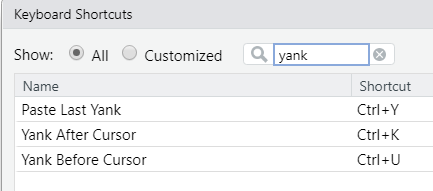
\includegraphics{./images/paste-AA3074D1.png}

\hypertarget{directory-tips}{%
\section{Directory tips}\label{directory-tips}}

When you need to type a path, can use file path auto-complete which can
be brought up by pressing the auto-completion shortcut (Tab or Ctrl +
Space) from a pair of double or single quotes.

Go back one directory, use ..

file\_create(``../test.R'')

From Packages 2e:

usethis::use\_package\_doc() and then list imports: e.g.

\begin{Shaded}
\begin{Highlighting}[]
\DocumentationTok{\#\# usethis namespace: start}
\CommentTok{\#\textquotesingle{} @import fs}
\CommentTok{\#\textquotesingle{} @import XLConnect}
\CommentTok{\#\textquotesingle{} @importFrom readxl read\_excel}
\CommentTok{\#\textquotesingle{} @importFrom tibble tibble}
\CommentTok{\#\textquotesingle{} @importFrom timeDate BoxingDay}
\DocumentationTok{\#\# usethis namespace: end}
\ConstantTok{NULL}
\end{Highlighting}
\end{Shaded}

In a central location. This approach keeps all (\textbf{importFrom?})
tags together, in a dedicated section of the package-level documentation
file (which can be created with usethis::use\_package\_doc()). This is
what use\_import\_from() implements. So, in R/pkg-package.R, you'll end
up with something like this:

\hypertarget{taking-screenshots-for-writing-.qmd-documents-like-this-one}{%
\section{Taking Screenshots for writing .qmd documents (like this
one)}\label{taking-screenshots-for-writing-.qmd-documents-like-this-one}}

\begin{itemize}
\item
  Images are taken using

  Press \textbf{Windows logo key + Shift + S} and paste in a .qmd file
  inside RStudio.
\end{itemize}

\hypertarget{resources}{%
\chapter{resources}\label{resources}}



\printindex

\end{document}
